%%==================================================================%%
%% Author : P�rez Ruiz, Alejandro                                   %%
%% Author : S�nchez Barreiro, Pablo                                 %%
%% Version: 1.1, 16/01/2011                                         %%                                                                                    %%                                                                  %%
%% Memoria del Proyecto Fin de Carrera                              %%
%% Domain Engineering/Architecture                                  %%
%%==================================================================%%

Un hogar inteligente posee una serie de dispositivos que se descomponen en \emph{sensores} y \emph{actuadores}. Los \emph{sensores} son los encargados de obtener los datos del elemento al que pertenecen, como por ejemplo, los grados que hace en una habitaci�n, la apertura que tiene una ventana... Los \emph{actuadores} se encargan de ejecutar las ordenes, por ejemplo que una persiana se abra o se cierre, la calefacci�n se encienda a unos determinados grados...

Tanto los sensores como los actuadores se encuentran conectados a un dispositivo central que los coordina, el cual se conoce como \emph{puerta de enlace} (en ingl�s, \emph{Gateway}). Dicho Gateway se encarga de leer los datos de los sensores, procesarlos y enviar las ordenes adecuadas a los actuadores. De igual modo, el Gateway recibe ordenes de los usuarios que son ejecutadas por los actuadores para modificar los elementos de la casa.

%%=====================================================================%%
%% HECHO(Pablo): Aqu� hace falta una figura describiendo la            %%
%%              arquitectura                                           %%
%% http://www.google.es/imgres?imgurl=http://www.fancybread.com/blog/images//mediator.jpg&imgrefurl=http://www.fancybread.com/blog/post.cfm/mediator-pattern-applied-to-javascript&h=273&w=316&sz=25&tbnid=x1f5CI5WvMYNzM:&tbnh=101&tbnw=117&prev=/search%3Fq%3DMediator%2BPattern%26tbm%3Disch%26tbo%3Du&zoom=1&q=Mediator+Pattern&hl=es&usg=__ZG2xo8qDKX8sPv-uWS_mDcE-zQo=&sa=X&ei=MnL7TZLvNcWYhQfkrYizAw&ved=0CEcQ9QEwBQ
%%=====================================================================%%
Por tanto, tal como se ve en la Figura~\ref{domain:fig:mediador}, el dise�o de nuestra arquitectura es una aplicaci�n concreta del patr�n de dise�o \emph{mediador}~\cite{gamma:1994}, donde el \emph{Gateway} ejercer el papel de mediador, y los diferentes sensores y actuadores son los distintos elementos a coordinar. El objetivo de este patr�n es extraer y encapsular en una �nica clase la l�gica de coordinaci�n de un conjunto de objetos que necesitan interaccionar entre ellos siguiendo reglas de coordinaci�n de cierta complejidad. Al encapsular esta l�gica en un �nico objeto, denominado \emph{mediador} , el dise�o de los diferentes objetos que deben interactuar, en nuestro caso sensores y actuadores,  se simplifica, ya que estos elementos ahora s�lo tienen que notificar eventos al mediador y recibir notificaciones del mismo. Del mismo modo, cualquier cambio en la l�gica de coordinaci�n de estos objetos afecta solo a la clase \emph{Mediador}, el \emph{Gateway} en nuestro caso, en lugar de a los diferentes objetos que toman parte en la interacci�n.
\begin{figure}[!h]
 \centering
 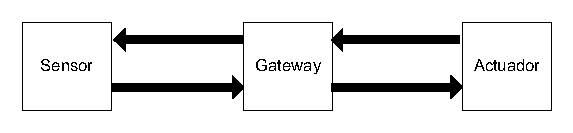
\includegraphics[width=.55\linewidth]{domainEngineering/images/Mediator.eps} \\
 \caption{Dise�o de la arquitectura a trav�s del patr�n de dise�o \emph{mediador}}
 \label{domain:fig:mediador}
\end{figure}

Adem�s de los sensores y actuadores, para que el usuario pueda controlar y visualizar el estado de los diversos dispositivos es necesario la creaci�n de una interfaz gr�fica que permita al usuario interactuar con el \emph{Gateway}.

Esta interfaz gr�fica tendr� que actualizar el estado de sus elementos cuando se producen cambios en los dispositivos. Para simplificar esta dependencia entre la interfaz gr�fica y el \emph{Gateway}, haremos uso del patr�n \emph{Observador}~\cite{gamma:1994} (\emph{Observer pattern}, en ingl�s). Para instanciar este patr�n, el \emph{Gateway} contendr� una lista por cada dispositivo que pueda ser observado. Los objetos interesados en ser notificados cada vez que dicho dispositivo cambie su estado se registrar�n o a�adir�n en dicha lista. De esta forma, cada vez que un dispositivo cambia de estado, el \emph{Gateway} notifica dicho cambio a todos los objetos registrados en la correspondiente lista de \emph{observadores}.

Finalmente, y dado que este proyecto no trabaja con actuadores y sensores reales, es necesario simular mediante software dichos dispositivos. Por ejemplo, deberemos simular variables tales como la temperatura percibida por los sensores, o el transcurso del tiempo del sistema. Para ello crearemos una interfaz gr�fica que juegue el papel de simulador, y permita al usuario interactuar con los dispositivos a simular as� como alterar diversas variables externas al sistema, como la temperatura.

Una vez definido el dise�o arquitect�nico b�sico, se desarrollan las iteraciones necesarias para completar la fase de ingenier�a del dominio. La siguiente secci�n describe los principios de dise�o seguidos para la construcci�n de dichas caracter�sticas. 